\documentclass{article}
\usepackage{graphics} 
\usepackage{hyperref}
\usepackage{fixltx2e}
\usepackage{amssymb}
\usepackage{tikz}

\author{Kevin Zollicoffer}
\title{Regression\\Lesson 4a}
\date{11/04/2013}

% no indents
\setlength\parindent{0pt}

\usepackage{Sweave}
\begin{document}
\maketitle
%\tableofcontents
\Sconcordance{concordance:Assignment4a.tex:Assignment4a.Rnw:%
1 8 1 1 0 11 1 1 2 1 0 1 2 4 1 1 2 19 0 1 2 3 1 1 2 1 0 4 1 3 0 1 2 2 1 %
1 2 1 0 1 1 33 0 2 2 117 0 1 2 6 0 1 2 1 1 5 0 1 2 1 1 6 0 1 2 4 1 1 10 %
9 0 1 2 2 1 1 2 23 0 1 1 27 0 1 3 2 1 2 2 4 1 1 2 24 0 1 1 27 0 1 3 1 1 %
2 2 4 1 1 2 24 0 1 1 27 0 1 3 1 1 2 2 7 1 1 3 8 0 1 2 8 1}


\section*{Introduction}
Regression assignment 4a using R
\\
\\
The complete source for this assigment is available on Github:
\\
\\
\url{https://github.com/zollie/PASS}

\section*{Problem 5.1}
\begin{Schunk}
\begin{Sinput}
> gpa <- read.csv("~/R/PASS/Regression/Assignment4a/collgpa.csv")
\end{Sinput}
\end{Schunk}
\subsection*{a}
\begin{Schunk}
\begin{Sinput}
> model <- lm(Gpa ~ Verb+Math, data=gpa)
> summary(model)
\end{Sinput}
\begin{Soutput}
Call:
lm(formula = Gpa ~ Verb + Math, data = gpa)

Residuals:
     Min       1Q   Median       3Q      Max 
-1.60273 -0.29620  0.09961  0.36998  0.54313 

Coefficients:
             Estimate Std. Error t value Pr(>|t|)    
(Intercept) -0.905450   0.606037  -1.494 0.143642    
Verb         0.027974   0.004939   5.664 1.79e-06 ***
Math         0.026139   0.006048   4.322 0.000112 ***
---
Signif. codes:  0 ‘***’ 0.001 ‘**’ 0.01 ‘*’ 0.05 ‘.’ 0.1 ‘ ’ 1

Residual standard error: 0.4938 on 37 degrees of freedom
Multiple R-squared:  0.5545,	Adjusted R-squared:  0.5304 
F-statistic: 23.03 on 2 and 37 DF,  p-value: 3.189e-07
\end{Soutput}
\begin{Sinput}
> stu <- rstudent(model)
\end{Sinput}
\end{Schunk}
\begin{Schunk}
\begin{Sinput}
> plot(gpa$Verb, stu)
\end{Sinput}
\end{Schunk}
\begin{Schunk}
\begin{Sinput}
> scatter.smooth(gpa$Verb, stu, span=.75)
\end{Sinput}
\end{Schunk}
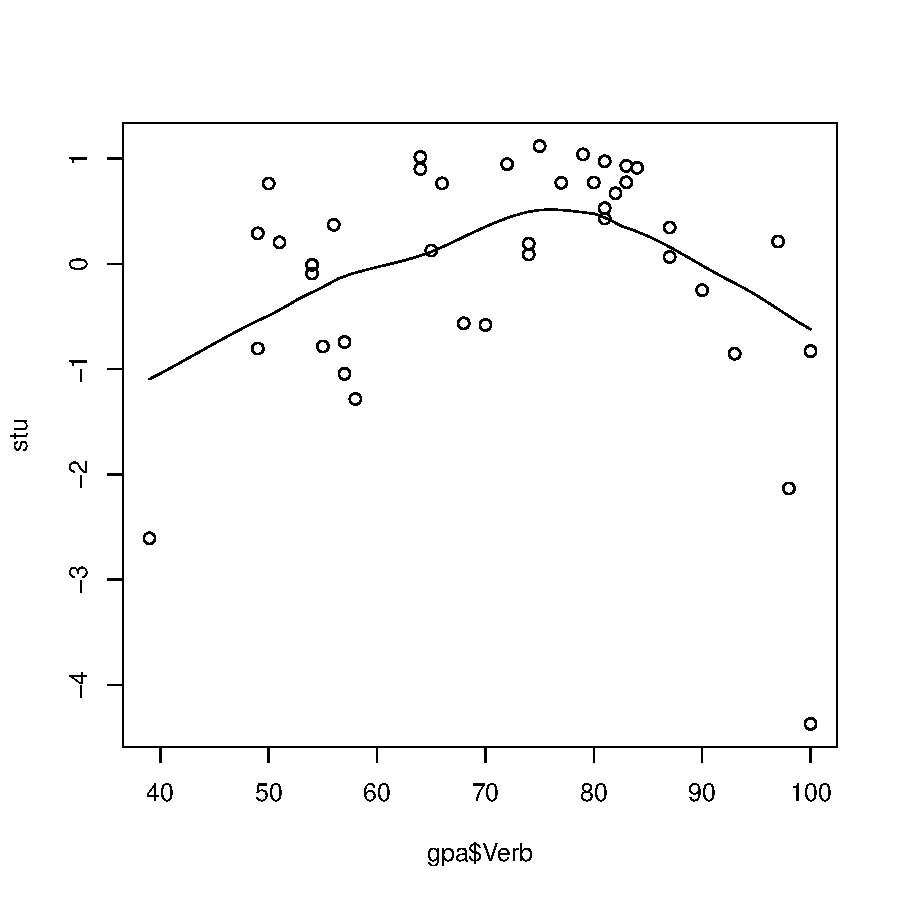
\includegraphics{Assignment4a-004}
\begin{Schunk}
\begin{Sinput}
> plot(gpa$Math, stu)
\end{Sinput}
\end{Schunk}
\begin{Schunk}
\begin{Sinput}
> scatter.smooth(gpa$Math, stu, span=.75)
\end{Sinput}
\end{Schunk}
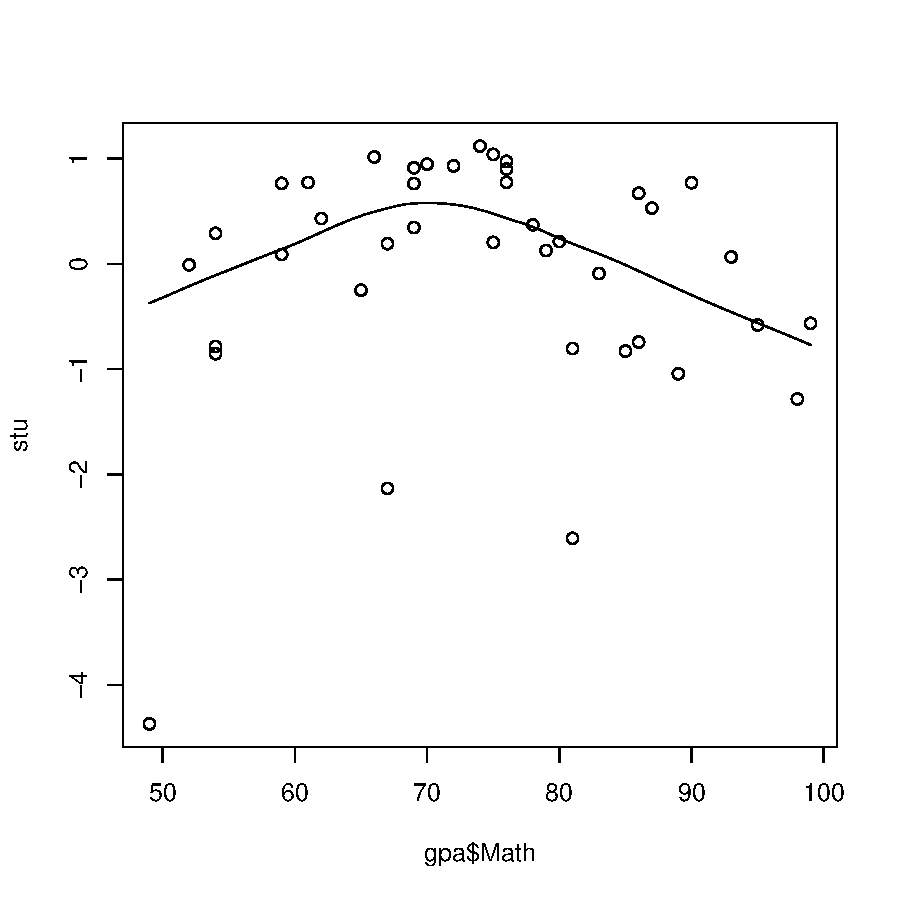
\includegraphics{Assignment4a-006}
\\
The zero mean assumption appears to be violated. Moreso by the verb residuals. 

\subsection*b
\begin{Schunk}
\begin{Sinput}
> modelb <- lm(Gpa ~ Verb+Math+Verb*Math+Verb**2+Math**2, data=gpa)
> summary(modelb)
\end{Sinput}
\begin{Soutput}
Call:
lm(formula = Gpa ~ Verb + Math + Verb * Math + Verb^2 + Math^2, 
    data = gpa)

Residuals:
     Min       1Q   Median       3Q      Max 
-0.86322 -0.19643  0.08819  0.29644  0.50905 

Coefficients:
              Estimate Std. Error t value Pr(>|t|)    
(Intercept)  5.3959500  1.7197528   3.138 0.003389 ** 
Verb        -0.0599174  0.0232608  -2.576 0.014249 *  
Math        -0.0610439  0.0232714  -2.623 0.012696 *  
Verb:Math    0.0012209  0.0003178   3.842 0.000477 ***
---
Signif. codes:  0 ‘***’ 0.001 ‘**’ 0.01 ‘*’ 0.05 ‘.’ 0.1 ‘ ’ 1

Residual standard error: 0.4215 on 36 degrees of freedom
Multiple R-squared:  0.6841,	Adjusted R-squared:  0.6577 
F-statistic: 25.98 on 3 and 36 DF,  p-value: 4.024e-09
\end{Soutput}
\begin{Sinput}
> stub <- rstudent(modelb)
> levb <- hatvalues(modelb)
> cookb <- cooks.distance(modelb)
> mean(stub)
\end{Sinput}
\begin{Soutput}
[1] -0.05527571
\end{Soutput}
\end{Schunk}
\begin{Schunk}
\begin{Sinput}
> plot(modelb)
\end{Sinput}
\end{Schunk}
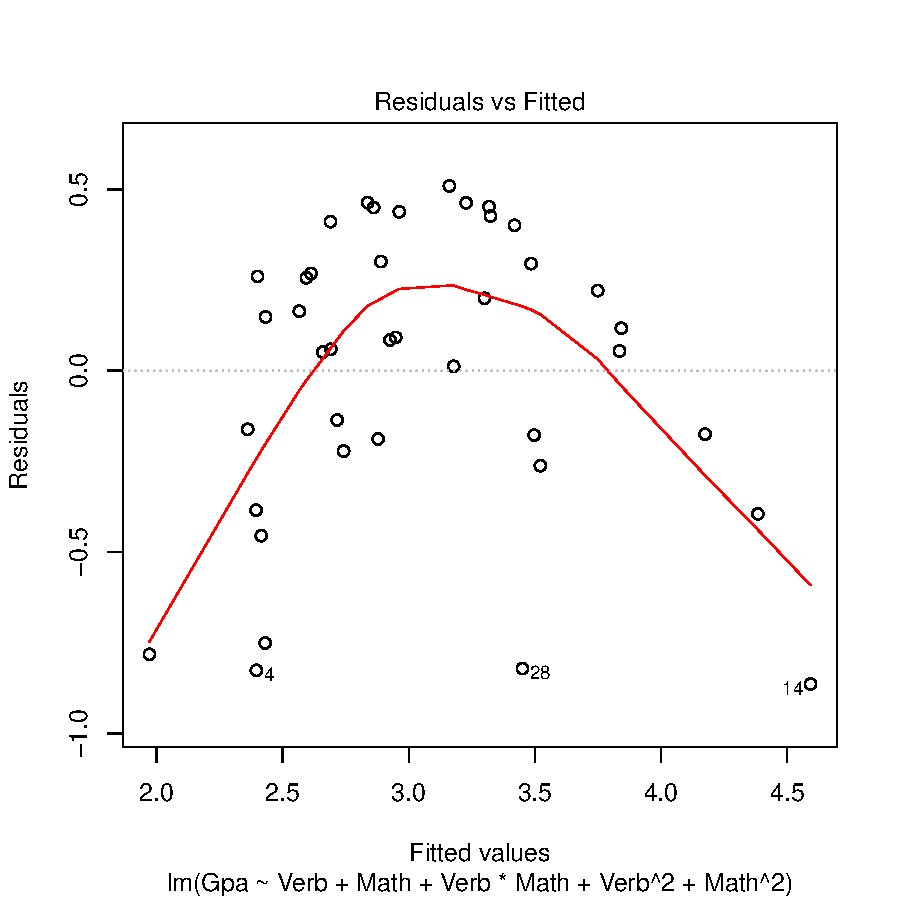
\includegraphics{Assignment4a-008}

The resdiuals may have a mean near 0, but the distribution does not appear uniform (linear). There appears to be curviture in the data with fat tails on the ends. I'm not sure that this data does not violate the zero mean assumption?
\subsection*c
\begin{Schunk}
\begin{Sinput}
> hist(stub)
\end{Sinput}
\end{Schunk}
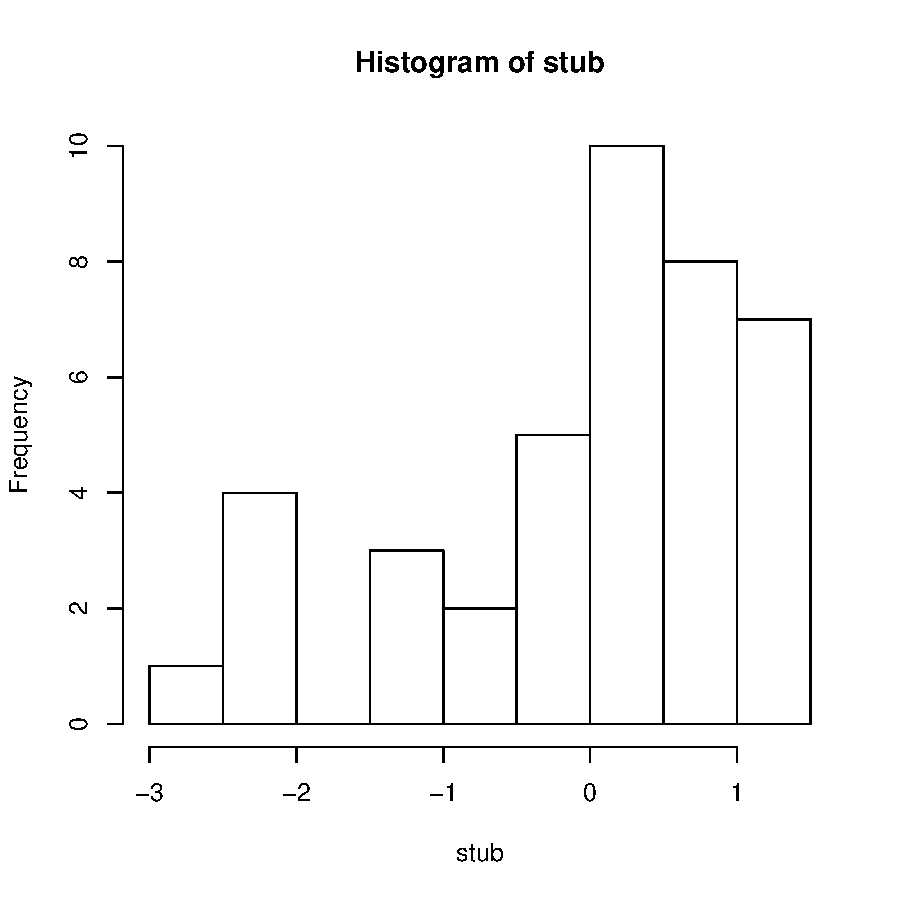
\includegraphics{Assignment4a-009}

This data is left skewed and does not appear normally distributed about the mean. 

\begin{Schunk}
\begin{Sinput}
> qqnorm(stub)
> qqline(stub)
\end{Sinput}
\end{Schunk}
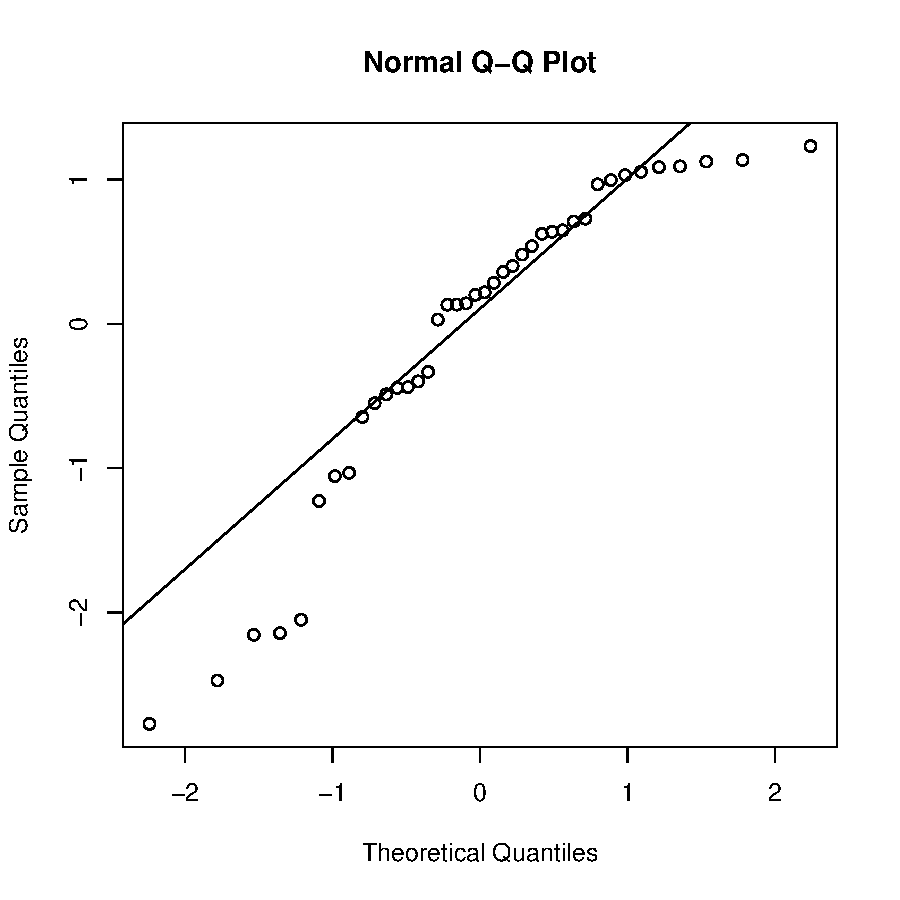
\includegraphics{Assignment4a-010}

The QQ-plot appears normal near the center of the data range but skewed $> +-$ Quantile 2. 

\subsection*d
Yes, observation 4 appears to be an outlier. This is based on (e) and (f) below. Please see below. 

\subsection*e
Observation 4 has the highest leverage. 

\begin{Schunk}
\begin{Sinput}
> plot(gpa$ID, levb)
\end{Sinput}
\end{Schunk}
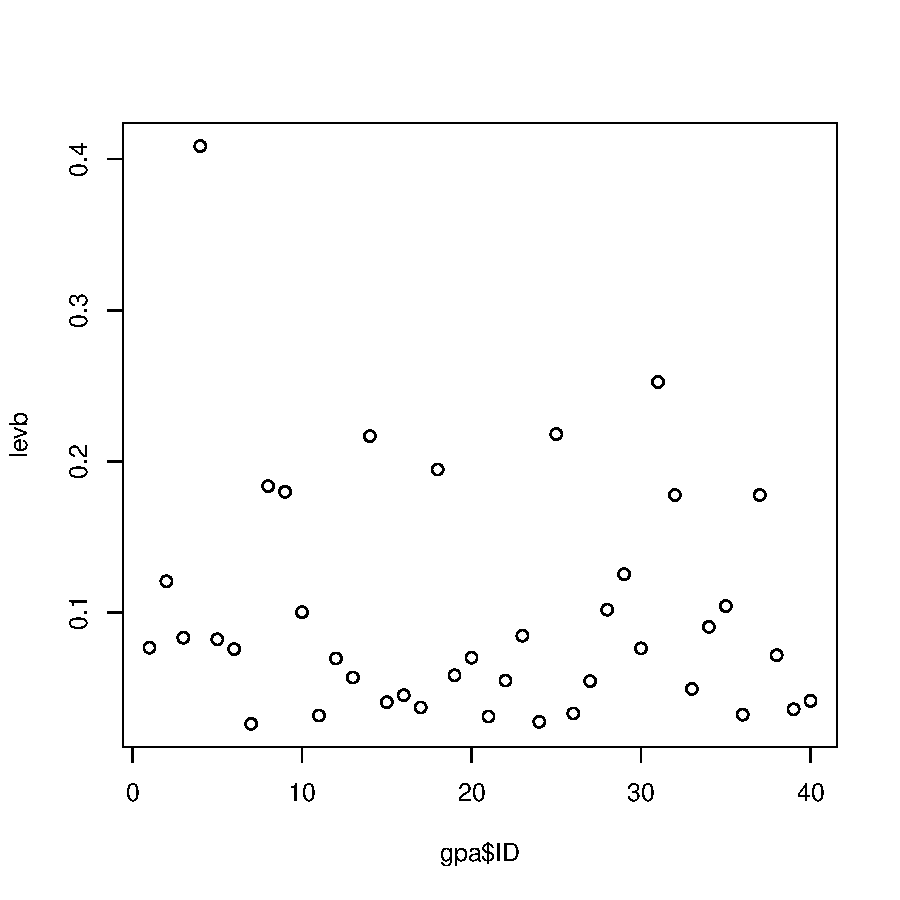
\includegraphics{Assignment4a-011}

\subsection*f
Observation 4 has the highest cook distance. This observation is removed, and the model recalculated below. 

\begin{Schunk}
\begin{Sinput}
> plot(gpa$ID, cookb)
\end{Sinput}
\end{Schunk}
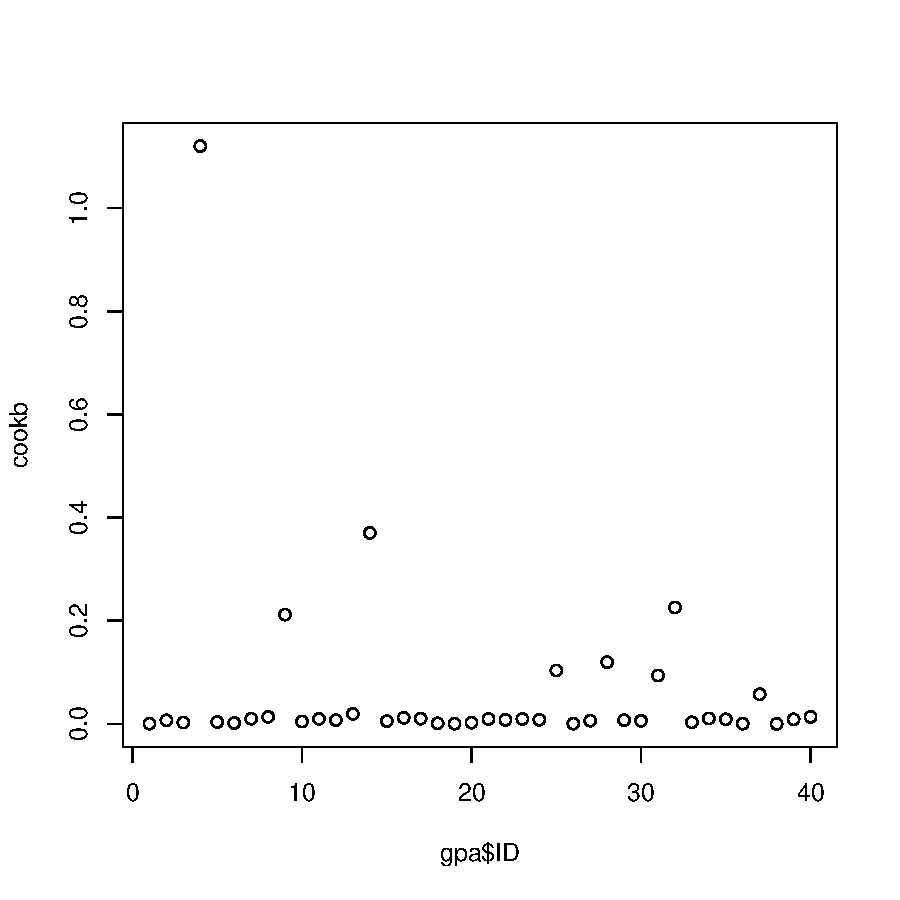
\includegraphics{Assignment4a-012}

\begin{Schunk}
\begin{Sinput}
> gpa2 <- gpa[-4,]
> modelb2 <- lm(Gpa ~ Verb+Math+Verb*Math+Verb**2+Math**2, data=gpa2)
> summary(modelb2)
\end{Sinput}
\begin{Soutput}
Call:
lm(formula = Gpa ~ Verb + Math + Verb * Math + Verb^2 + Math^2, 
    data = gpa2)

Residuals:
     Min       1Q   Median       3Q      Max 
-1.03419 -0.20544  0.09268  0.30412  0.47827 

Coefficients:
             Estimate Std. Error t value Pr(>|t|)  
(Intercept)  2.926399   1.813044   1.614   0.1155  
Verb        -0.020127   0.025732  -0.782   0.4394  
Math        -0.029711   0.024173  -1.229   0.2272  
Verb:Math    0.000716   0.000344   2.081   0.0448 *
---
Signif. codes:  0 ‘***’ 0.001 ‘**’ 0.01 ‘*’ 0.05 ‘.’ 0.1 ‘ ’ 1

Residual standard error: 0.3871 on 35 degrees of freedom
Multiple R-squared:  0.7089,	Adjusted R-squared:  0.6839 
F-statistic:  28.4 on 3 and 35 DF,  p-value: 1.718e-09
\end{Soutput}
\begin{Sinput}
> stub2 <- rstudent(modelb2)
> levb2 <- hatvalues(modelb2)
> cookb2 <- cooks.distance(modelb2)
> mean(stub2)
\end{Sinput}
\begin{Soutput}
[1] -0.04922247
\end{Soutput}
\end{Schunk}

\begin{Schunk}
\begin{Sinput}
> plot(modelb2)
\end{Sinput}
\end{Schunk}
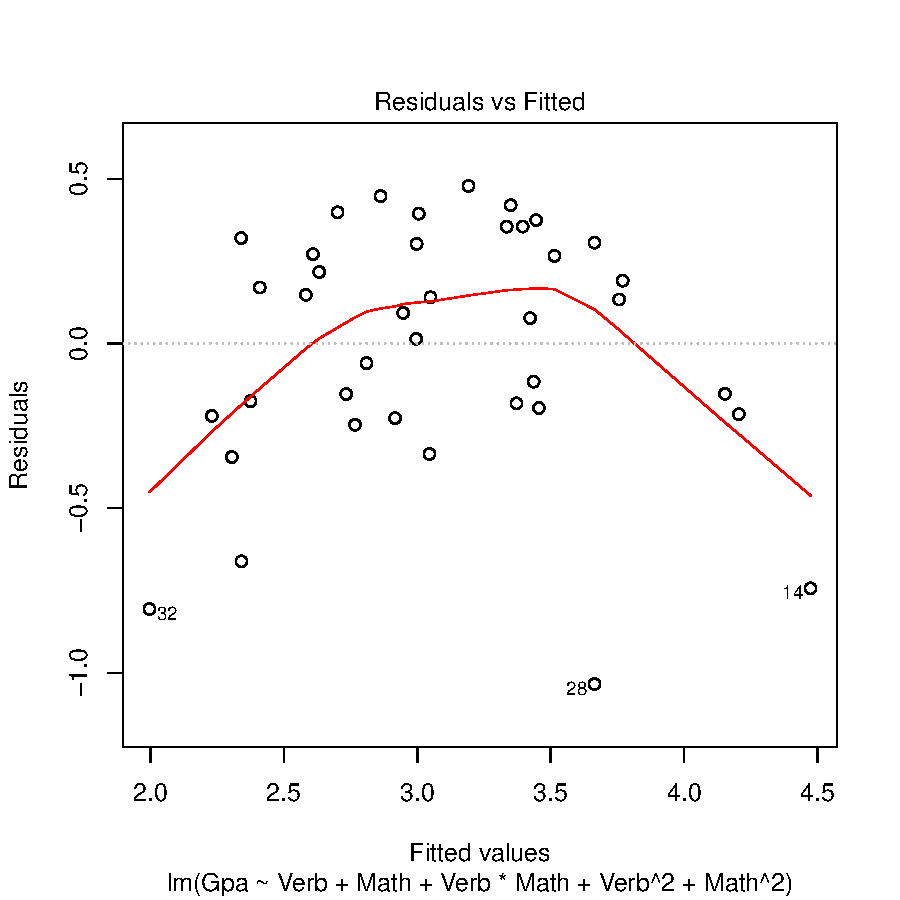
\includegraphics{Assignment4a-014}

\begin{Schunk}
\begin{Sinput}
> hist(stub2)
\end{Sinput}
\end{Schunk}
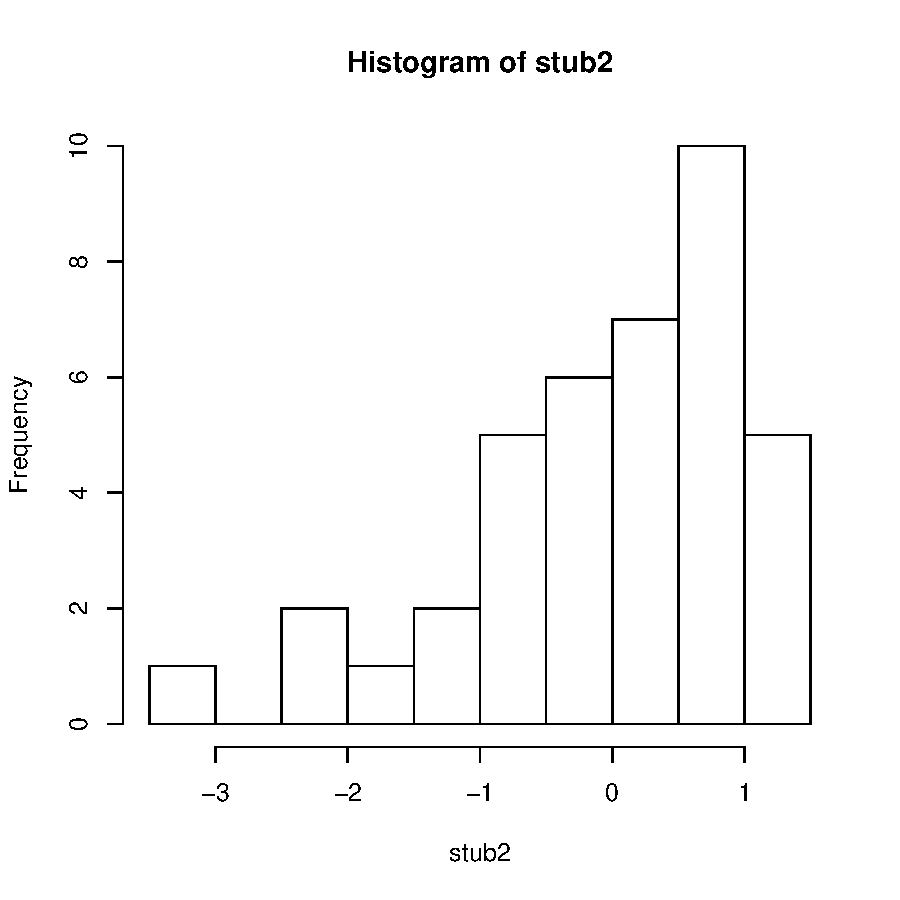
\includegraphics{Assignment4a-015}

\begin{Schunk}
\begin{Sinput}
> plot(gpa2$ID, cookb2)
\end{Sinput}
\end{Schunk}
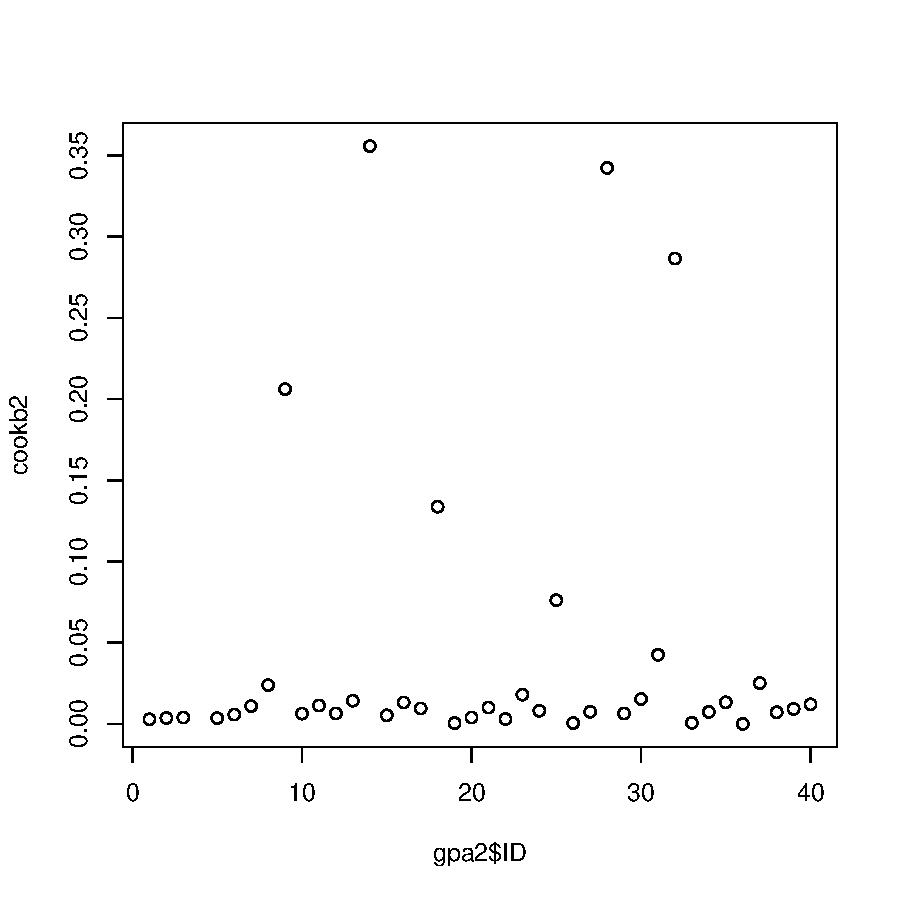
\includegraphics{Assignment4a-016}

\section*{Problem 5.7}
Below is the regression model developed for problem 5.7. It has an $R^2$ of .9472 and standard error of 10.05

\begin{Schunk}
\begin{Sinput}
> rest <- read.csv("~/R/PASS/Regression/Assignment4a/restaurant.csv")
> rest$Region = factor(rest$Region)
> rest$DSw <- NULL
> rest$DNw <- NULL
> fit <- lm(Profit ~ Cov+Fco+Oco+Lco+Region+Cov*Fco*Lco*Region+Region*Lco*Oco, data=rest)
> summary(fit)
\end{Sinput}
\begin{Soutput}
Call:
lm(formula = Profit ~ Cov + Fco + Oco + Lco + Region + Cov * 
    Fco * Lco * Region + Region * Lco * Oco, data = rest)

Residuals:
     Min       1Q   Median       3Q      Max 
-22.6886  -4.2094  -0.6898   5.0272  23.8367 

Coefficients:
                       Estimate Std. Error t value Pr(>|t|)
(Intercept)           1.910e+02  2.389e+02   0.799    0.426
Cov                   1.903e+00  2.326e+01   0.082    0.935
Fco                  -6.171e-01  2.094e+00  -0.295    0.769
Oco                  -1.979e+00  1.289e+00  -1.535    0.128
Lco                  -2.552e+00  2.664e+00  -0.958    0.341
RegionNW              6.160e+02  6.567e+02   0.938    0.351
RegionSW             -2.223e+02  4.325e+02  -0.514    0.609
Cov:Fco               7.498e-02  1.427e-01   0.526    0.600
Cov:Lco               2.209e-01  2.315e-01   0.954    0.342
Fco:Lco              -9.587e-03  2.053e-02  -0.467    0.642
Cov:RegionNW         -7.634e+01  5.713e+01  -1.336    0.185
Cov:RegionSW          4.308e+01  3.626e+01   1.188    0.238
Fco:RegionNW         -1.266e+00  4.348e+00  -0.291    0.772
Fco:RegionSW          1.837e-01  3.479e+00   0.053    0.958
Lco:RegionNW         -6.629e+00  7.308e+00  -0.907    0.367
Lco:RegionSW          7.713e-01  5.088e+00   0.152    0.880
Oco:RegionNW         -1.566e+00  1.977e+00  -0.792    0.431
Oco:RegionSW          3.534e-01  1.630e+00   0.217    0.829
Oco:Lco               1.436e-02  1.271e-02   1.130    0.262
Cov:Fco:Lco          -4.593e-04  1.233e-03  -0.372    0.710
Cov:Fco:RegionNW      3.600e-01  3.123e-01   1.153    0.252
Cov:Fco:RegionSW     -2.162e-01  2.296e-01  -0.942    0.349
Cov:Lco:RegionNW      7.368e-01  6.118e-01   1.204    0.232
Cov:Lco:RegionSW     -3.440e-01  3.884e-01  -0.886    0.378
Fco:Lco:RegionNW      1.255e-02  4.536e-02   0.277    0.783
Fco:Lco:RegionSW      1.279e-02  3.645e-02   0.351    0.727
Oco:Lco:RegionNW      2.055e-02  2.064e-02   0.995    0.322
Oco:Lco:RegionSW     -7.247e-03  1.615e-02  -0.449    0.655
Cov:Fco:Lco:RegionNW -3.638e-03  3.194e-03  -1.139    0.258
Cov:Fco:Lco:RegionSW  1.433e-03  2.205e-03   0.650    0.517

Residual standard error: 10.05 on 90 degrees of freedom
Multiple R-squared:  0.9472,	Adjusted R-squared:  0.9301 
F-statistic: 55.63 on 29 and 90 DF,  p-value: < 2.2e-16
\end{Soutput}
\end{Schunk}

\end{document}
